\section{\textsc{MobileGym++} Playground}
\label{sec:mobilegym++}
\label{sec:method}

\subsection{A gap in controllable commercial applications}
\label{sec:mgpp-env}

Mobile agents are increasingly moving toward real-world workflows across commercial applications, such as travel booking on Trip and online shopping on Taobao, where tasks are often long-horizon and grounded in real user needs. However, training and evaluation environments for such commercial applications remain largely missing. 
Real-device or Android-emulator setups introduce login friction, irreversible side effects, and costly reset procedures that make large-scale training impractical~\citep{rawles2025androidworld,kong2026mobileworld}. Prior simulated-app work, meanwhile, covers only a narrow range of commercial domains~\citep{wu2026mobilegym,trivedi2024appworld}.
As a result, mobile agents have limited opportunities to practice and be evaluated on realistic mobile-use scenarios.

We built MobileGym++, a browser-hosted mobile environment that supports realistic commercial workflows in controllable simulated applications. The runtime extends MobileGym~\citep{wu2026mobilegym}, preserving its advantages in reset and programmatic evaluation while substantially expanding domain coverage, the number and richness of applications, and support for native cross-app interaction. Observations consist of raw screen pixels; there is no accessibility tree and the agent cannot read business state directly. Device state is fully serializable, enabling deterministic reset and lightweight parallel instantiation. We newly built 35 high-fidelity commercial applications in this round, bringing the total to 63 installable clients spanning travel, shopping, finance, content, social, office, and local services. Each application maintains persistent business state---orders, budgets, itineraries---that evolves through interaction and supports programmatic task verification.
Table~\ref{tab:mgpp-stack-compare} compares MobileGym++ with existing mobile agent environments.

\begin{table*}[t]
\caption{Comparison of mobile agent environments across scale, interaction, and controllability. \ding{51} denotes supported, \ding{55} unsupported, and $\sim$ indicates limited system level cross-app interaction support in MobileGym. \# Comm. Apps and \# Tasks denote the number of covered commercial apps and benchmark tasks, respectively;
Detailed application statistics are provided in Appendix~\ref{app:mgpp-apps}. 
MobileGym++ provides diverse, high-fidelity commercial-style applications with full controllability, while introducing an experimental app-native tool interface.}
\label{tab:mgpp-stack-compare}
\centering
\scriptsize
\setlength{\tabcolsep}{3.0pt}
\renewcommand{\arraystretch}{1.16}
\resizebox{\linewidth}{!}{%
\begin{tabular}{@{}l l c c c c c c@{}}
\toprule
\multirow{2}{*}[-0.6ex]{Environment} 
& \multirow{2}{*}[-0.6ex]{Platform}
& \multicolumn{2}{c}{Scale} 
& \multicolumn{3}{c}{Interaction} 
& \multirow{2}{*}[-0.6ex]{\shortstack{Full\\Controllability}} \\
\cmidrule(lr){3-4} 
\cmidrule(lr){5-7}
& & \# Comm. Apps & \# Tasks  
& Cross-app & GUI & App-native Tools 
& \\
\midrule
AppWorld~\citep{trivedi2024appworld} & API & 9 & 750  
& \ding{51} & \ding{55} & \ding{55} & \ding{51} \\

AndroidLab~\citep{xu2025androidlab} & Emulator & 5 & 138  
& \ding{55} & \ding{51} & \ding{55} & \ding{55} \\

AndroidWorld~\citep{rawles2025androidworld} & Emulator & 0 & 116  
& \ding{51} & \ding{51} & \ding{55} & \ding{55} \\

SPA-Bench~\citep{chen2024spa} & Real-device & 58 & 340  
& \ding{51} & \ding{51} & \ding{55} & \ding{55} \\

MobileWorld~\citep{kong2026mobileworld} & Emulator & 4 & 201  
& \ding{51} & \ding{51} & \ding{55} & \ding{55} \\

MobileGym~\citep{wu2026mobilegym} & Simulator & 12 & 256  
& $\sim$ & \ding{51} & \ding{55} & \ding{51} \\

\textbf{MobileGym++ (ours)} & Simulator & \textbf{35} & \textbf{215}  
& \greencheck & \greencheck & \greencheck & \greencheck \\

\bottomrule
\end{tabular}%
}
\vspace{2pt}
\end{table*}

\subsection{35 high-fidelity commercial applications}
\label{sec:mgpp-apps}

The 35 applications are structurally faithful replicas of their real-world counterparts. Construction starts from the source application's data schema and interaction graph, specified before any interface is rendered, so business-state richness and navigation depth are architectural properties of each replica. 
Human annotators then iteratively compare each replica against the live application and refine both functionality and visual fidelity until the state transitions, and interface details closely match the reference application (Appendix~\ref{app:mgpp-build}).
Every delivered app is checked in two ways before tasks are written on it: a coverage check maps each declared interaction to its implementation, and a replay of the core flows confirms that each transition produces the declared state change.
Across these clients, the median application exposes 37 routes, 166 interactive actions, and 86 page transitions, with a median interaction depth of 3 from the home screen. Relative to the 12 prior MobileGym business apps retained in the same environment, the newly built clients reach $1.48\times$ the interactive actions and $1.91\times$ the page transitions, as shown in Figure~\ref{fig:mgpp-app-scale}.


\begin{figure}[t]
\centering
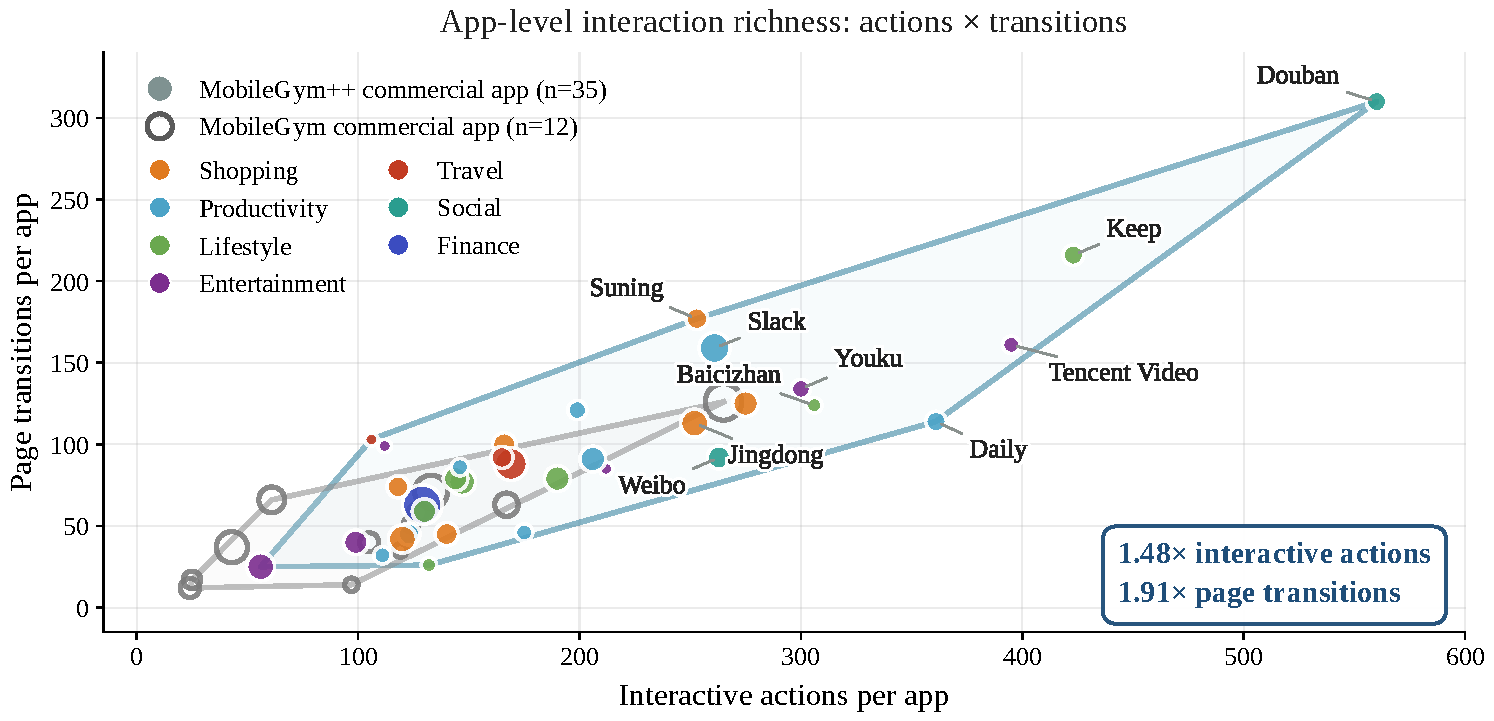
\includegraphics[width=0.85\linewidth]{figures/fig_app_richness_act_trans.pdf}
\caption{
App-level interaction richness. Each marker denotes one app, positioned by its interactive actions and page transitions; marker size reflects the number of Bench tasks using that app. Our new apps reach 1.48$\times$ more actions and 1.91$\times$ more transitions.
}
\label{fig:mgpp-app-scale}
\end{figure}


\subsection{Realistic cross-application workflows}
\label{sec:mgpp-crossapp}

Many real-world mobile workflows span multiple applications, requiring agents to retrieve information in one app, carry it across application boundaries, and complete an action in another. Single-application benchmarks cannot capture this behavior.

MobileGym++ extends simulated mobile use with explicit cross-application interaction mechanisms, including clipboard transfer, app-to-app sharing, payment redirection, and media selection.
All applications run on a shared, resettable device whose full state can be serialized and restored across episodes. Each app maintains its own business objects---such as orders, expenses, and itineraries---which evolve through interaction. These mechanisms allow information and actions to flow across application boundaries, enabling realistic multi-app workflows rather than isolated single-app tasks.

\subsection{Hybrid GUI and app-native tool use}
\label{sec:mgpp-tools}


Computer use is shifting beyond GUI-only interaction toward hybrid graphical and code interfaces.
We bring this idea to mobile use through an experimental setting in which applications selectively expose app-native tools alongside their GUIs. 
Unlike prior mobile settings with external tools~\citep{kong2026mobileworld}, our tools expose native app functions and operate on the same state as the GUI.

We follow a simple, principled design for tool construction: each tool exposes a structured lookup or write operation over an application's own business objects, while preserving semantic equivalence with the corresponding GUI interaction. A tool call and its GUI counterpart therefore modify the same persistent state and are evaluated by the same terminal condition.
This enables controlled comparison of the two interaction channels without changing tasks, initialization, or success criteria.
We implement over 300 such tools across more than 50 applications, including system clients such as Clock and Notes; tool depth varies by app, from a few search and lookup functions to more than ten read and write operations. All benchmark tasks remain solvable through GUI-only interaction, while hybrid agents can interleave GUI actions and app-native tool calls within the same task.



\subsection{\textsc{MobileGym++ Bench}}
\label{sec:mgpp-bench}

MobileGym++ Bench enables reliable evaluation of mobile agents in commercial-style applications through resettable environments and programmatic verification over application-level business states. Unlike existing benchmarks that rely on device-level signals~\citep{rawles2025androidworld,kong2026mobileworld}, MobileGym++ Bench evaluates whether agents achieve the intended changes in application business objects. Furthermore, the same task suite supports both GUI-only and hybrid GUI–tool interaction, enabling controlled comparison between the two settings. See details in Appendix~\ref{app:mgpp-bench}.

\textbf{Task Design.}
The primary source of difficulty is commercial navigation and information flow. A single-app task requires the agent to locate, filter, and fill fields across a deep page stack before a business object is written. A cross-application task further requires a live value from another application's store to be identified, carried across the application boundary, and written into the correct field. Instructions are phrased as user goals and do not name widgets, tools, or checker fields; the terminal is a write in the application's own business state.

\textbf{Scale and Composition.}
The benchmark comprises 215 tasks across seven business domains, including 109 single-app, 74 two-app, 27 three-app, and 5 four-app tasks. Tasks are balanced across applications and business objects to avoid domination by a small subset of clients.


\textbf{Evaluation Protocol.}
Each task specifies a user goal, a bound initial state, and a programmatic checker over the before/after diff of application business state. The checker does not inspect the trajectory or screenshots and does not rely on a model judge. GUI-only and Hybrid are evaluated on the same tasks, initial states, and checks. The primary metric is success rate.
